\documentclass[journal]{IEEEtran}
\usepackage[a5paper, margin=10mm]{geometry}
%\usepackage{lmodern} % Ensure lmodern is loaded for pdflatex
\usepackage{tfrupee} % Include tfrupee package


\setlength{\headheight}{1cm} % Set the height of the header box
\setlength{\headsep}{0mm}     % Set the distance between the header box and the top of the text


%\usepackage[a5paper, top=10mm, bottom=10mm, left=10mm, right=10mm]{geometry}

%
\setlength{\intextsep}{10pt} % Space between text and floats

\makeindex


\usepackage{cite}
\usepackage{amsmath,amssymb,amsfonts,amsthm}
\usepackage{algorithmic}
\usepackage{graphicx}
\usepackage{textcomp}
\usepackage{xcolor}
\usepackage{txfonts}
\usepackage{listings}
\usepackage{enumitem}
\usepackage{mathtools}
\usepackage{gensymb}
\usepackage{comment}
\usepackage[breaklinks=true]{hyperref}
\usepackage{tkz-euclide} 
\usepackage{listings}
\usepackage{multicol}
\usepackage{xparse}
\usepackage{gvv}
%\def\inputGnumericTable{}                                 
\usepackage[latin1]{inputenc}                                
\usepackage{color}                                            
\usepackage{array}                                            
\usepackage{longtable}                                       
\usepackage{calc}                                             
\usepackage{multirow}                                         
\usepackage{hhline}                                           
\usepackage{ifthen}                                               
\usepackage{lscape}
\usepackage{tabularx}
\usepackage{array}
\usepackage{float}
\usepackage{ar}
\usepackage[version=4]{mhchem}


\newtheorem{theorem}{Theorem}[section]
\newtheorem{problem}{Problem}
\newtheorem{proposition}{Proposition}[section]
\newtheorem{lemma}{Lemma}[section]
\newtheorem{corollary}[theorem]{Corollary}
\newtheorem{example}{Example}[section]
\newtheorem{definition}[problem]{Definition}
\newcommand{\BEQA}{\begin{eqnarray}}
\newcommand{\EEQA}{\end{eqnarray}}

\theoremstyle{remark}


\begin{document}
\bibliographystyle{IEEEtran}
\onecolumn

\title{12.249}
\author{INDHIRESH S- EE25BTECH11027}
\maketitle


\renewcommand{\thefigure}{\theenumi}
\renewcommand{\thetable}{\theenumi}

\textbf{Question}. A plane contains the following three points: $\Vec{P}(2, 1, 5), \Vec{Q}(-1, 3, 4)$ and $\Vec{R}(3, 0, 6)$. The vector perpendicular to the above plane can be represented as\\
\textbf{Solution}:\\
Let us solve the given equation theoretically and then verify the solution computationally. \\
Given points are:
\begin{align}
 \Vec{P}=\myvec{2\\1\\5}\;\;,\Vec{Q}=\myvec{-1\\3\\4}\;\;and\;\;\Vec{R}=\myvec{3\\0\\6}
\end{align}
Now finding two vectors in the plane:

\begin{align}
 \Vec{P}\Vec{Q}=\myvec{-3\\2\\-1}
\end{align}
\begin{align}
\Vec{P}\Vec{R}=\myvec{1\\-1\\1}
\end{align}
Now the required vector be $\Vec{n}$
\begin{align}
\Vec{n}=\Vec{P}\Vec{Q}\times\Vec{P}\Vec{R}
\end{align}
Let
\begin{align}
    \Vec{A}=\Vec{P}\Vec{Q}\;\;and\;\;\Vec{B}=\Vec{P}\Vec{R}
\end{align}
Then
\begin{align}
    \Vec{n}=\Vec{A}\times\Vec{B}
\end{align}

\begin{align}
\Vec{A}\times\Vec{B}=\myvec{\mydet{\Vec{A_{23}}\Vec{B_{23}}}\\\\\mydet{\Vec{A_{31}} \Vec{B_{31}}}\\\\\mydet{\Vec{A_{12}} \Vec{B_{12}}}}
\end{align}

\begin{align}
 \mydet{\Vec{A_{23}}\Vec{B_{23}}}=\mydet{2&-1\\-1&1}=1
\end{align}

\begin{align}
 \mydet{\Vec{A_{31}} \Vec{B_{31}}}=-\mydet{-3&-1\\1&1}=2
\end{align}

\begin{align}
 \mydet{\Vec{A_{12}} \Vec{B_{12}}}=\mydet{-3&2\\1&-1}=1
\end{align}

\begin{align}
  \Vec{A}\times\Vec{B}=\myvec{1\\2\\1}
\end{align}
\begin{align}
   \Vec{n}=\myvec{1\\2\\1}
\end{align}



From the figure it is clearly verified that the theoretical solution matches with the computational solution.\\
\begin{figure}[h]
    \centering
    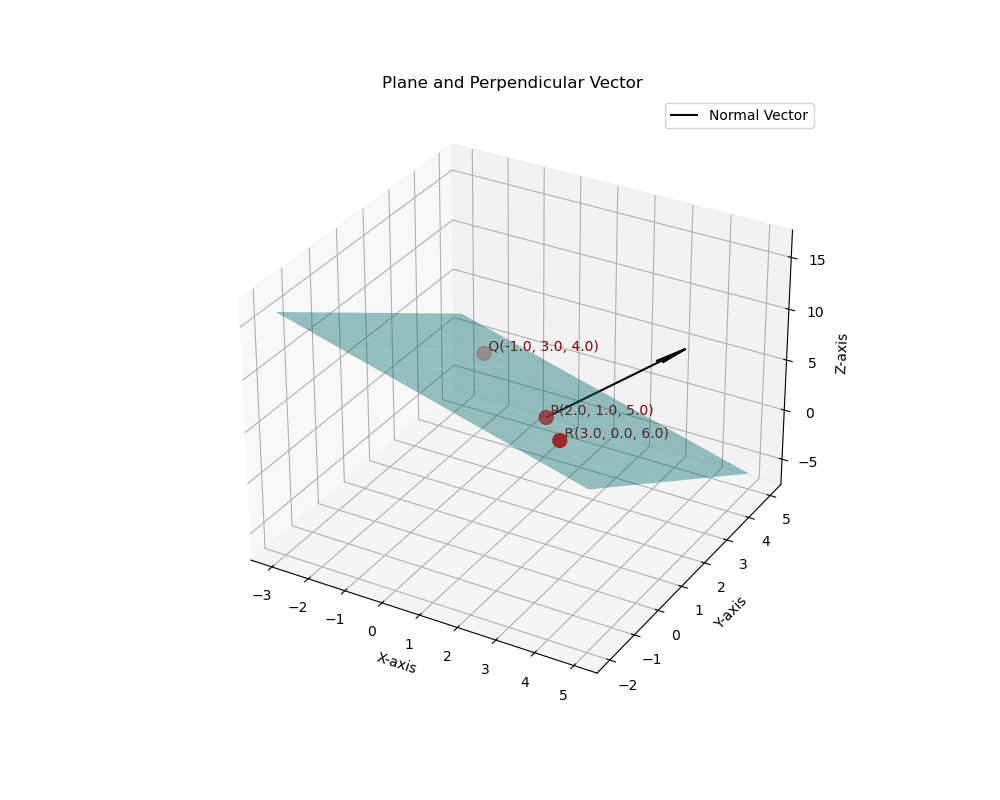
\includegraphics[height=0.5\textheight, keepaspectratio]{figs/figure1.png}
    \label{figure_1}
\end{figure}

\end{document}